\chapter{Dark Matter}
\label{sec:dm}

As a theory of the fundamental particles and forces of nature, the Standard Model should also help explain physics at the largest scales.
The $\Lambda$CDM model best explains all current cosmological observations including the structure of the cosmic microwave background; the abundances of hydrogren, helium, and lithium; the large-scale structure in the distribution of galaxies, and the accelerating expansion of the universe.
However, the latest results from the Planck collaboration show that bayronic matter (matter consisting of various combinations of protons, neutrons, and electrons) only contributes $\sim$5\% of the total energy of the universe, with radiation (photons and relativistic neutrinos) contributing less than a hundredth of a percent.

The remaining 95\% of energy comes from just two sources: $\sim$27\% from non-relativistic non-baryonic matter referred to as dark matter and $\sim$68\% from an unknown form of energy that permeates all of space referred to as dark energy.
Current observations show that dark energy is uniform in space and time producing a similar effect to that of the cosmological constant in the Einstein field equations of general relavity.
Not much else is known about dark energy, although there are many experiments attempting to discover additional properties.
The work in this thesis shall focus on trying to explain dark matter.

Dark matter cannot be explained by the 17 particles of the Standard Model (see Section~\ref{sec:dm_cand}), yet its gravitational effects have been observed in many circumstances.
The rest of this chapter will cover the astrophysical evidence for dark matter (Sections~\ref{sec:dm_astro} and~\ref{sec:dm_relic}), various dark matter candidates (Section~\ref{sec:dm_cand}), and non-collider searches for dark matter (Section~\ref{sec:dm_search}) before concluding with a discussion of the dark matter models investigated in this thesis (Section~\ref{sec:dm_simp}).

\section{Astrophysical Evidence}
\label{sec:dm_astro}

All existing evidence for dark matter comes from astrophysical observations of its gravitational effects on the universe at various length scales.
We shall focus on four different sources of evidence: the average velocity of galaxies in clusters, the rotation curves of spiral galaxies, strong gravitational lensing, and merging galactic clusters. The evidence presented here is not exhaustive, see Reference~\ref{Roos10} for more detail. % https://arxiv.org/pdf/1001.0316.pdf

\subsection{Galactic Clusters}
\label{sec:dm_clusters}

Galactic clusters are the largest gravitational bound systems, with the orbital velocities of the individual clusters determined by the total gravitional mass of the cluster. Applying the Virial Theorem gives the explicit relation
\begin{equation}
  v^2 = \frac{GM}{2r},
\end{equation}
where $v$ is the average orbital velocity of a galaxy in the cluster, $r$ is the average separation between galaxies in the cluster, $M$ is the total gravitational mass of the cluster, and $G$ is the Newtonian constant of gravitation.
In 1933, Fritz Zwicky measured the average orbtial velocity of the Coma clustered and discovered that it was a factor of ten larger than the observed visible mass of the Coma cluster, leading to the conclusion that the majority of the cluster consisted of non-luminous matter.
Today studies show that stars only contribute 1\% of the total cluster mass, with a hot, baryonic intracluster medium and dark matter contributing the remaining 14\% and 85\% of the total cluster mass, respectively.

\subsection{Galactic Rotation Curves}
\label{sec:dm_curves}

Spiral galaxies are stable gravitational bound systems with stars and interstellar gas rotating around the galactic center in nearly circular orbits in a single plane.
For these galaxies, the orbit of an individual star is stable when the gravitational force acting on the star balances the centripetal acceleration of the star.
With this condition, the expected stellar velocity $v$ is a function of distance $r$ from the galatic center given by
\begin{equation}
  v = \sqrt{\frac{GM(r)}{r}}
\end{equation}
where $M(r)$ is the total gravitational mass inside radius $r$.
Thus, past a certain critical radius $r_c$, the stellar velocity should fall with as $r^{1/2}$ as the mass of the galaxy is no longer increasing.
% https://arxiv.org/pdf/0907.1912.pdf

In 1980, Vera Rubin and Kent Ford observed that instead of decreasing at distances outside the visible galaxy, the stellar velocity stayed constant out to a very great distance, necessitating an additional non-luminous source of mass. % http://adsabs.harvard.edu/doi/10.1086/158003
The most common explanation for this missing mass is the existence of an isotropic dark matter halo surrounding the galaxy.
With the inclusion of interstellar gas, the total mass inside radius $r$ is given by
\begin{equation}
  M(r) = 4 \pi \int_0^r \text{d}r' (r')^2 \Big[\rho_{\text{S}}(r') + \rho_{\text{g}}(r') + \rho_{\text{DM}}(r') \Big],
\end{equation}
where $\rho_{\text{S}}$, $\rho_{\text{g}}$, and $\rho_{\text{DM}}$ are the density profiles of the stars, interstellar gas, and dark matter in the galaxy, respectively.
Once these densities have been specified, it is possible to plot the fraction of the total stellar velocity due to each mass source as a function of distance from the galactic center.

Figure~\ref{fig:rotation_curves} shows the results of doing this using the observed stellar and interstellar mass density profiles and the expected density from an isotropic dark matter halo for two different spiral galaxies.
In both cases, this reproduces the observed flat galactic rotation curve incredibly well, lending strong support for the existence of galactic dark matter halos. 

\begin{figure}[htbp]
  \centering
  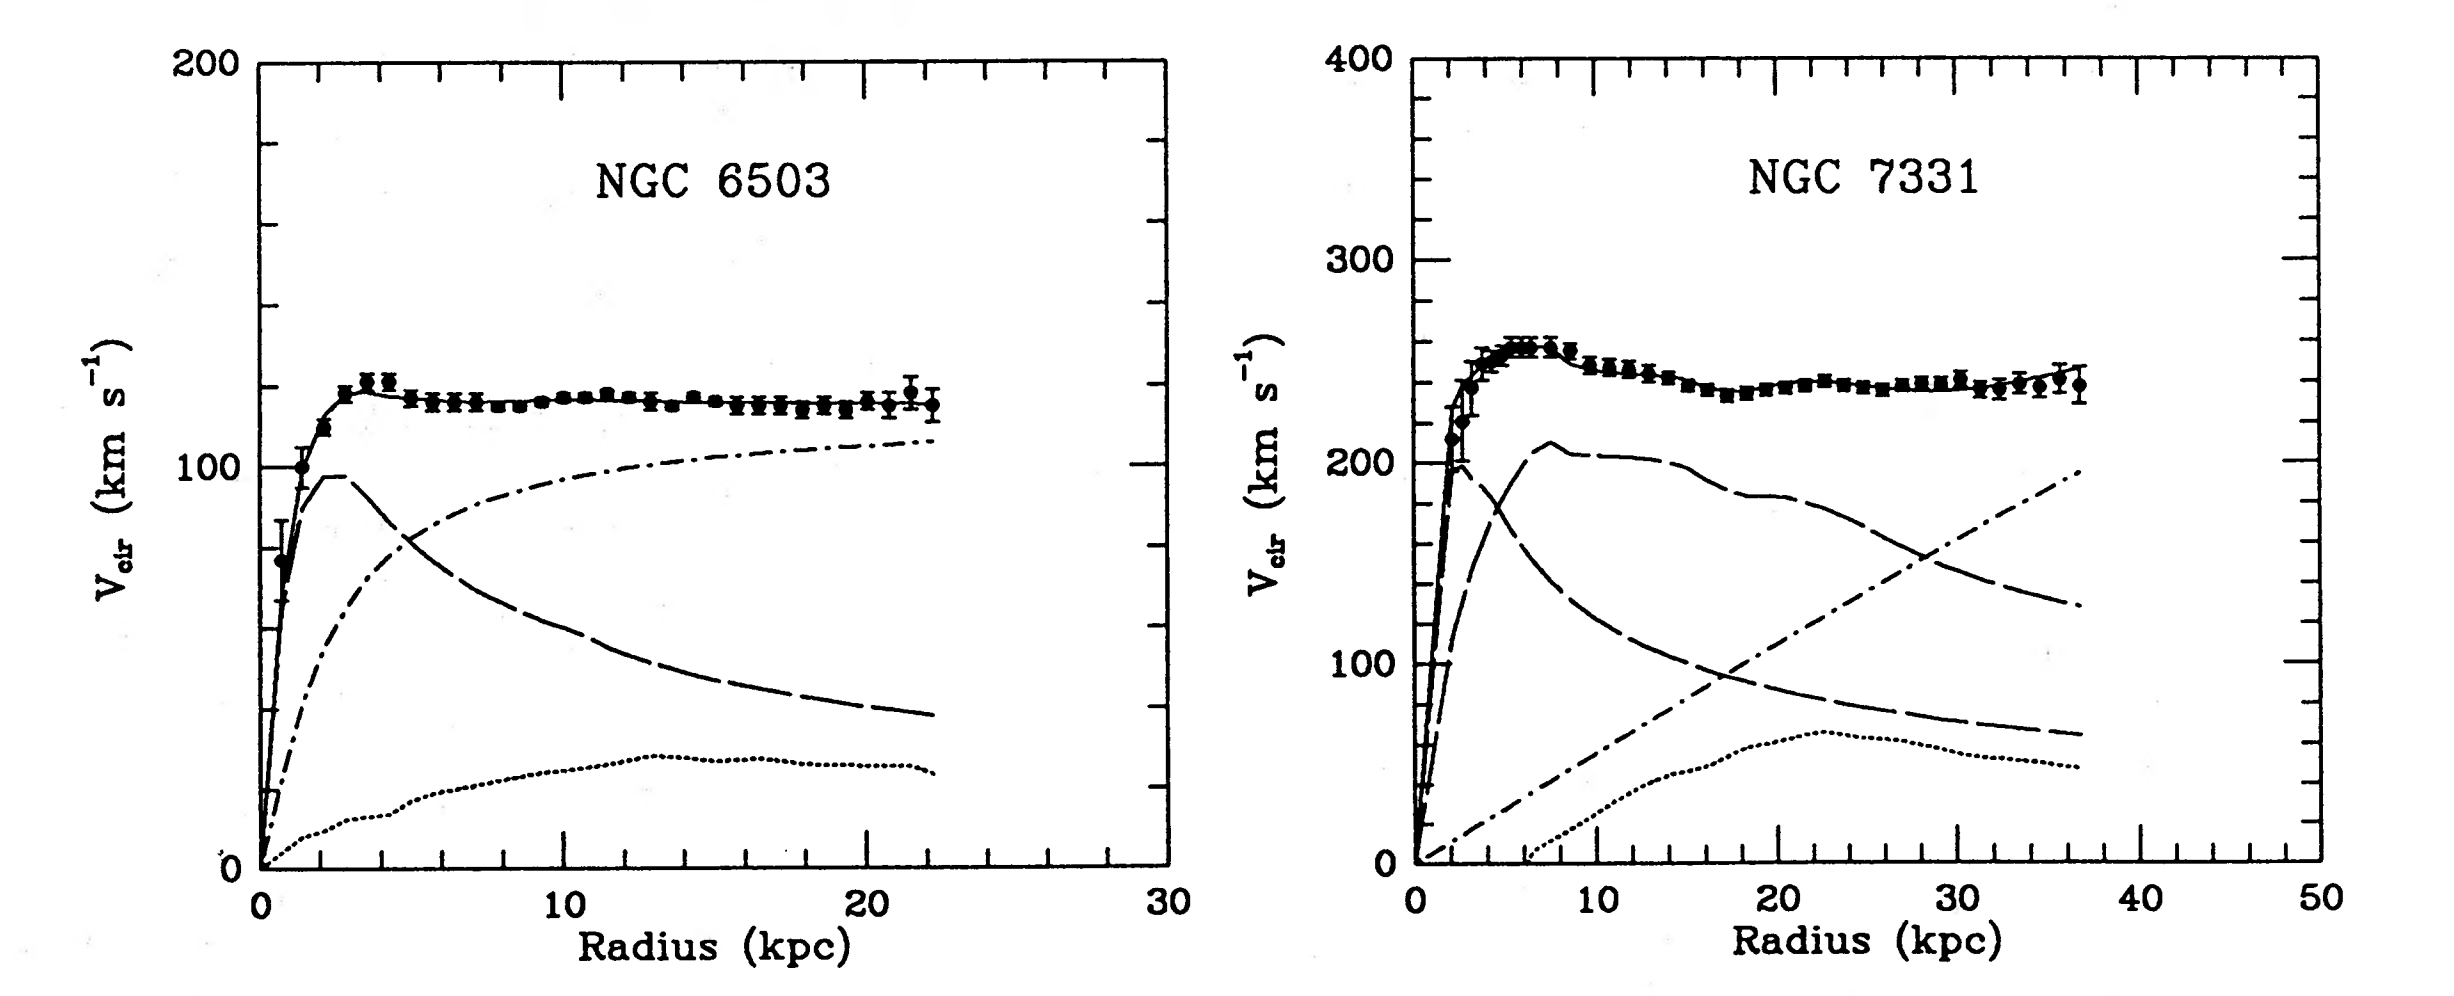
\includegraphics[width=0.85\textwidth]{DarkMatter/Figures/rotation_curves.png}
  \caption{
    The observed (points) and fitted (solid line) rotation curves for two sample galaxies.
    The fit consists of three components: the stellar component (dashed), the interstellar gas (dotted), and the dark matter halo (dash-dotted).
    Reprinted from Reference~\cite{}. % http://adsabs.harvard.edu/abs/1991MNRAS.249..523B
  }
  \label{fig:rotation_curves}
\end{figure}

\subsection{Gravitational Lensing}
\label{sec:dm_lensing}

As a consequence of Einstein's equivalence principle, a massive body will deflect light, a phenomenon know as gravitational lensing.
In the language of general relativity, this means that the photons take the path given by the geodesic lines following the curvature of space-time due to the massive body.
For most observations of gravitational lensing due to astrophysical bodies, the physical size of the lensing object is much smaller than the distance between observer, lens, and source allowing us to use the thin lens approximation.
Approximating the lens as a planar distribution of matter, the angular deflection is given by 
\begin{equation}
  \vec \alpha (\vec x) = \frac{4G}{c^2} \int \text{d}^2 x' \frac{\vec x - \vec {x'}}{\abs{\vec x - \vec{x'}}^2} 
  \int \text{d} z \rho(\vec{x'}, z)
\end{equation}
where $\vec x$ is a two-dimensional vector in the plane of the lens, $z$ is the perpendicular distance from the plane of the lens, and  $\rho$ is the three dimensional density.
If the source is treated as a point mass, this reduces to
\begin{equation}
  \alpha = \frac{ 4 G} {c^2} \cdot \frac{M}{b}
\end{equation}
where $b = \abs{\vec x - \vec{x'}}$ is the impact parameter and $M$ is the total mass of the object.
% The angle of deflection from the path traveled in the absence of a deflecting body is directly proportional to the mass of the deflecting body.
Thus, measuring the angle of deflection due to gravitional lensing around an astrophysical object provides an independent measurement of the total mass of the body which can be compared against the mass of the luminous objects in the body.
% https://arxiv.org/pdf/1001.1739.pdf

\begin{figure}[htbp]
  \centering
  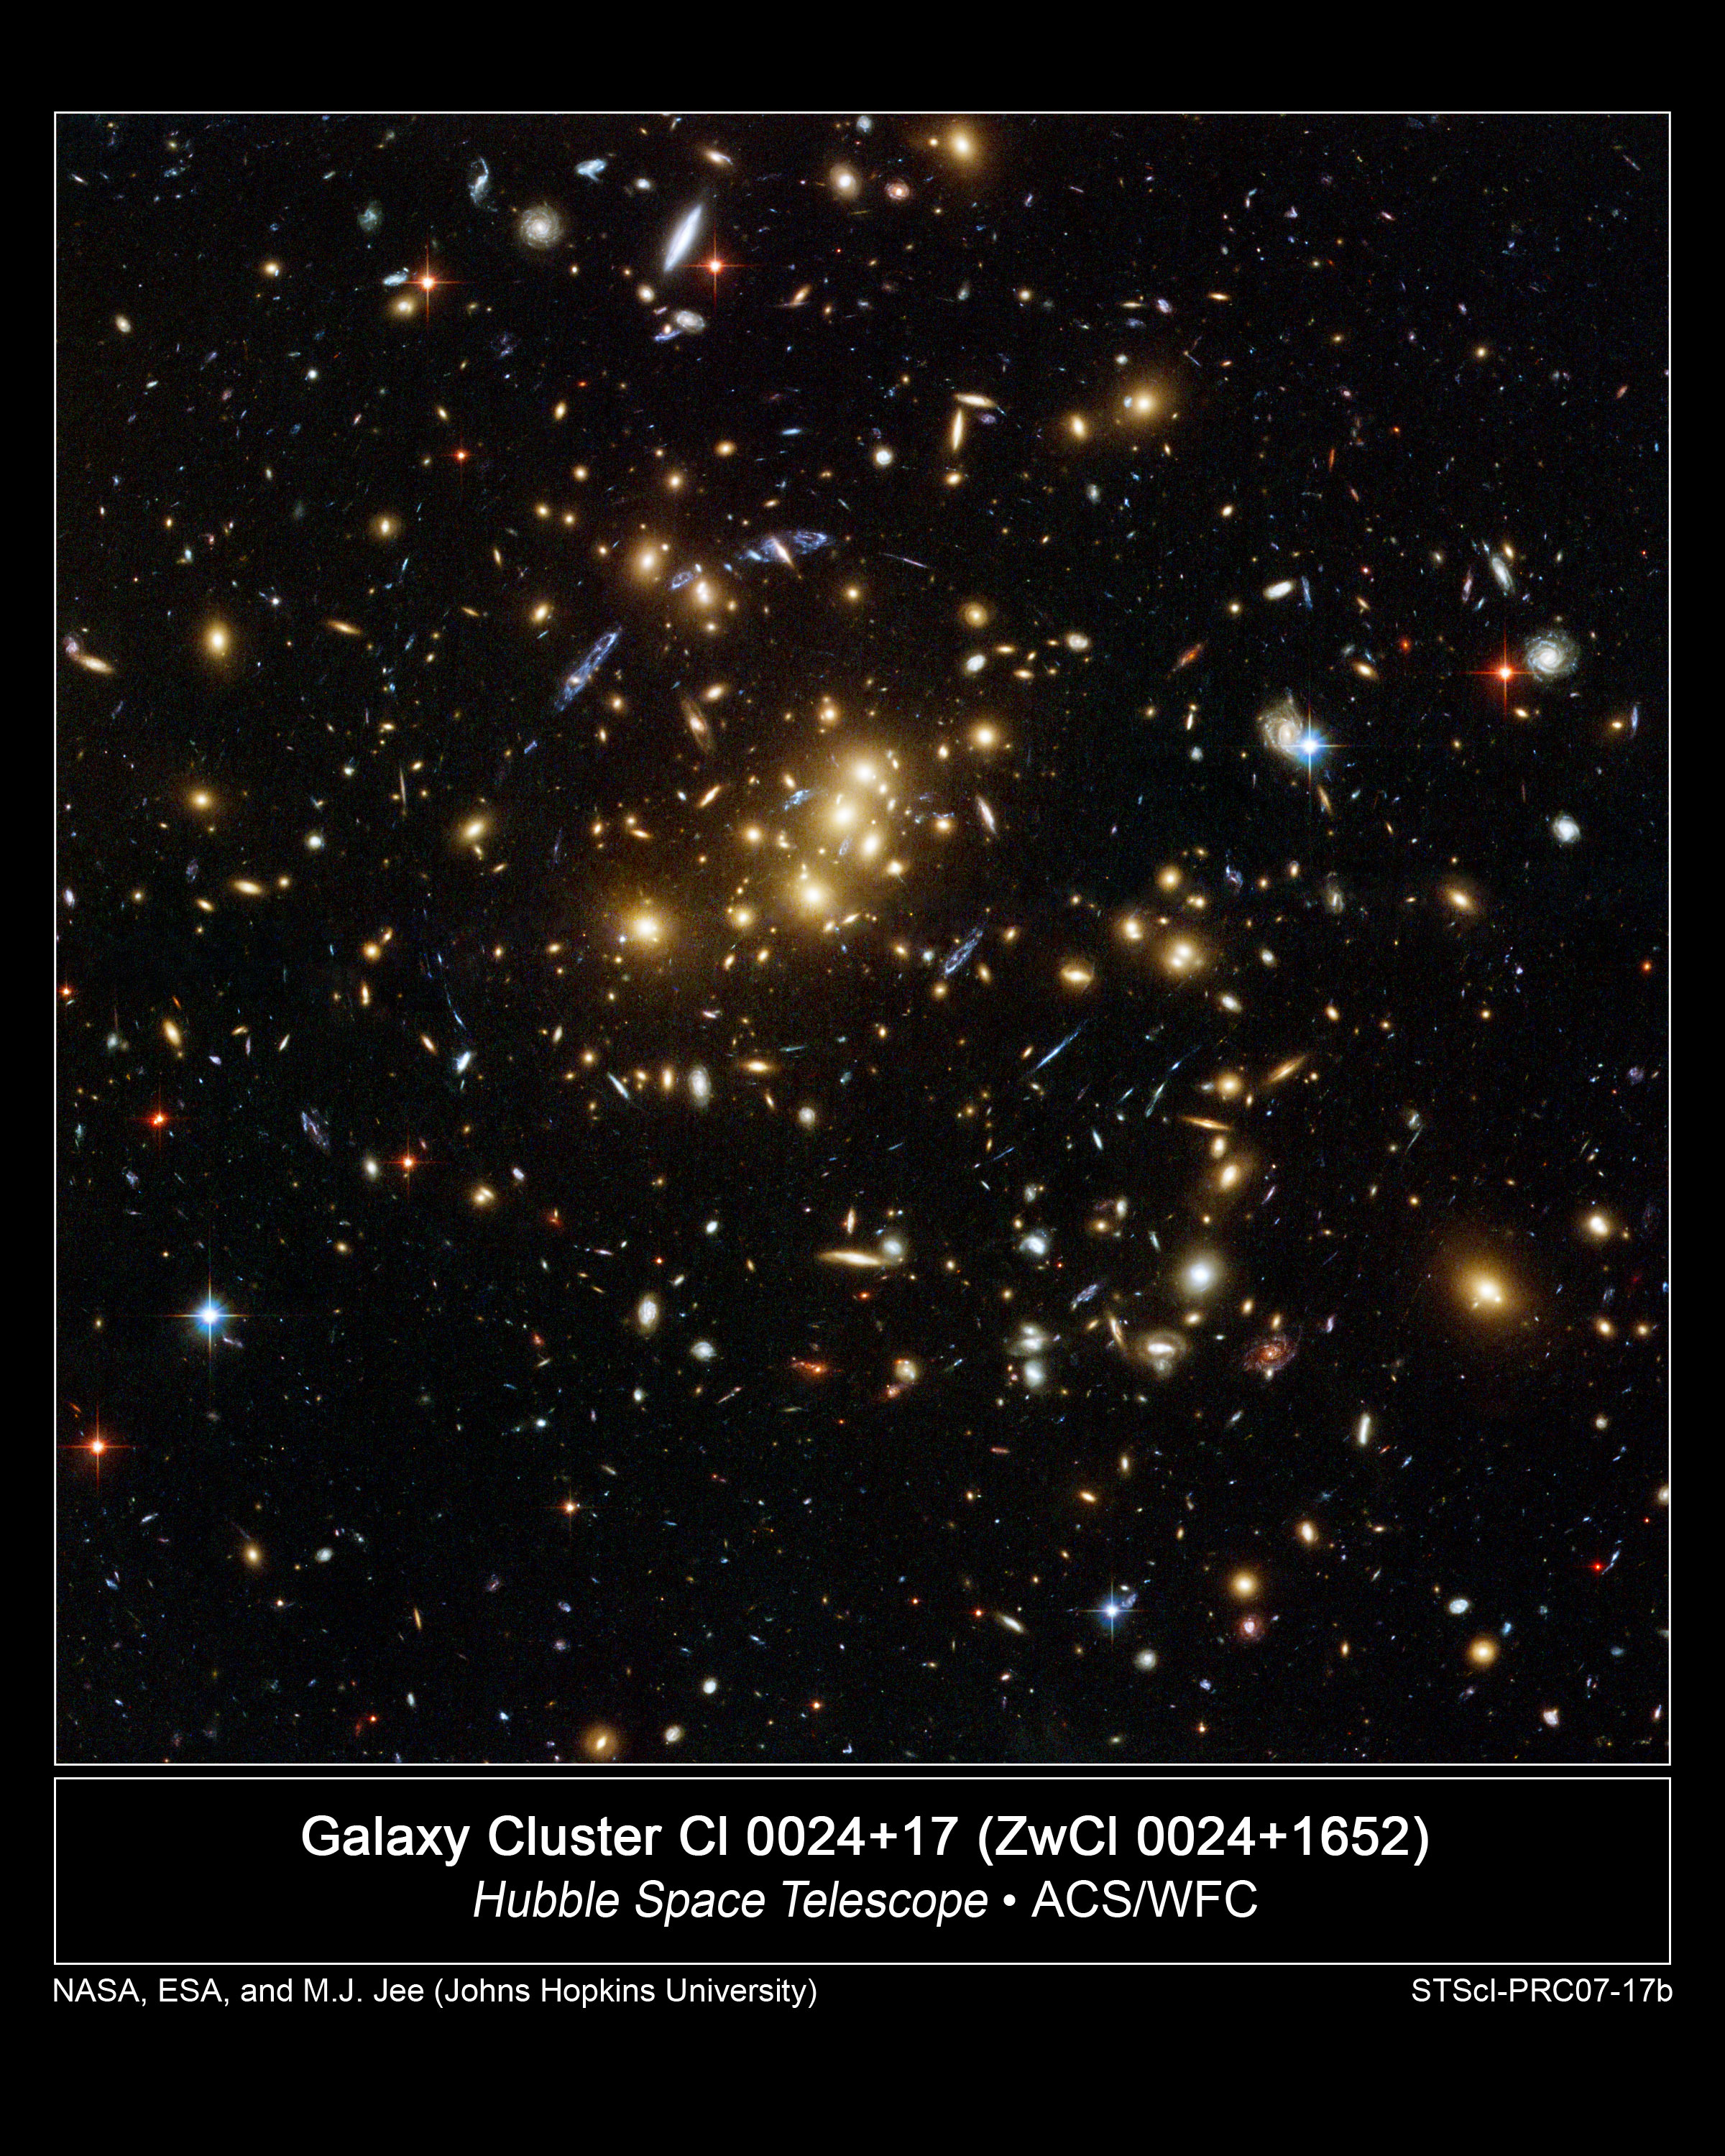
\includegraphics[width=\textwidth]{DarkMatter/Figures/strong_lensing.jpg}
  \caption{
    Strong gravitational lensing around galaxy cluster CL0024+17, consisting of the graviationally bound yellow, elliptical galaxies.
    The elongated blue objects are from much more distant galaxies behind the cluster which are distorted into arcs due to gravitational lensing from the dark matter halo surrounding the cluster.
    Figure credit:  NASA, ESA, M.J. Jee and H. Ford (Johns Hopkins University)
  }
  \label{fig:strong_lensing}
\end{figure}

Depending on the mass of the deflecting body and impact parameter, the size of deflection can fall into three different regimes.
The first of these is called strong lensing where the curving of space-time is so strong that light can travel multiple paths around the lens and still reach the observer.
If the source is directly behind a circular lens, light travels around all sides of the lens and appears as an Einstein ring, while if the source is offset or the lens is non-circular, the source will instead appear in multiple locations as if viewed from slightly different angles.
An example of strong lensing is shown in Figure~\ref{fig:strong_lensing}.

\begin{figure}[htbp]
  \centering
  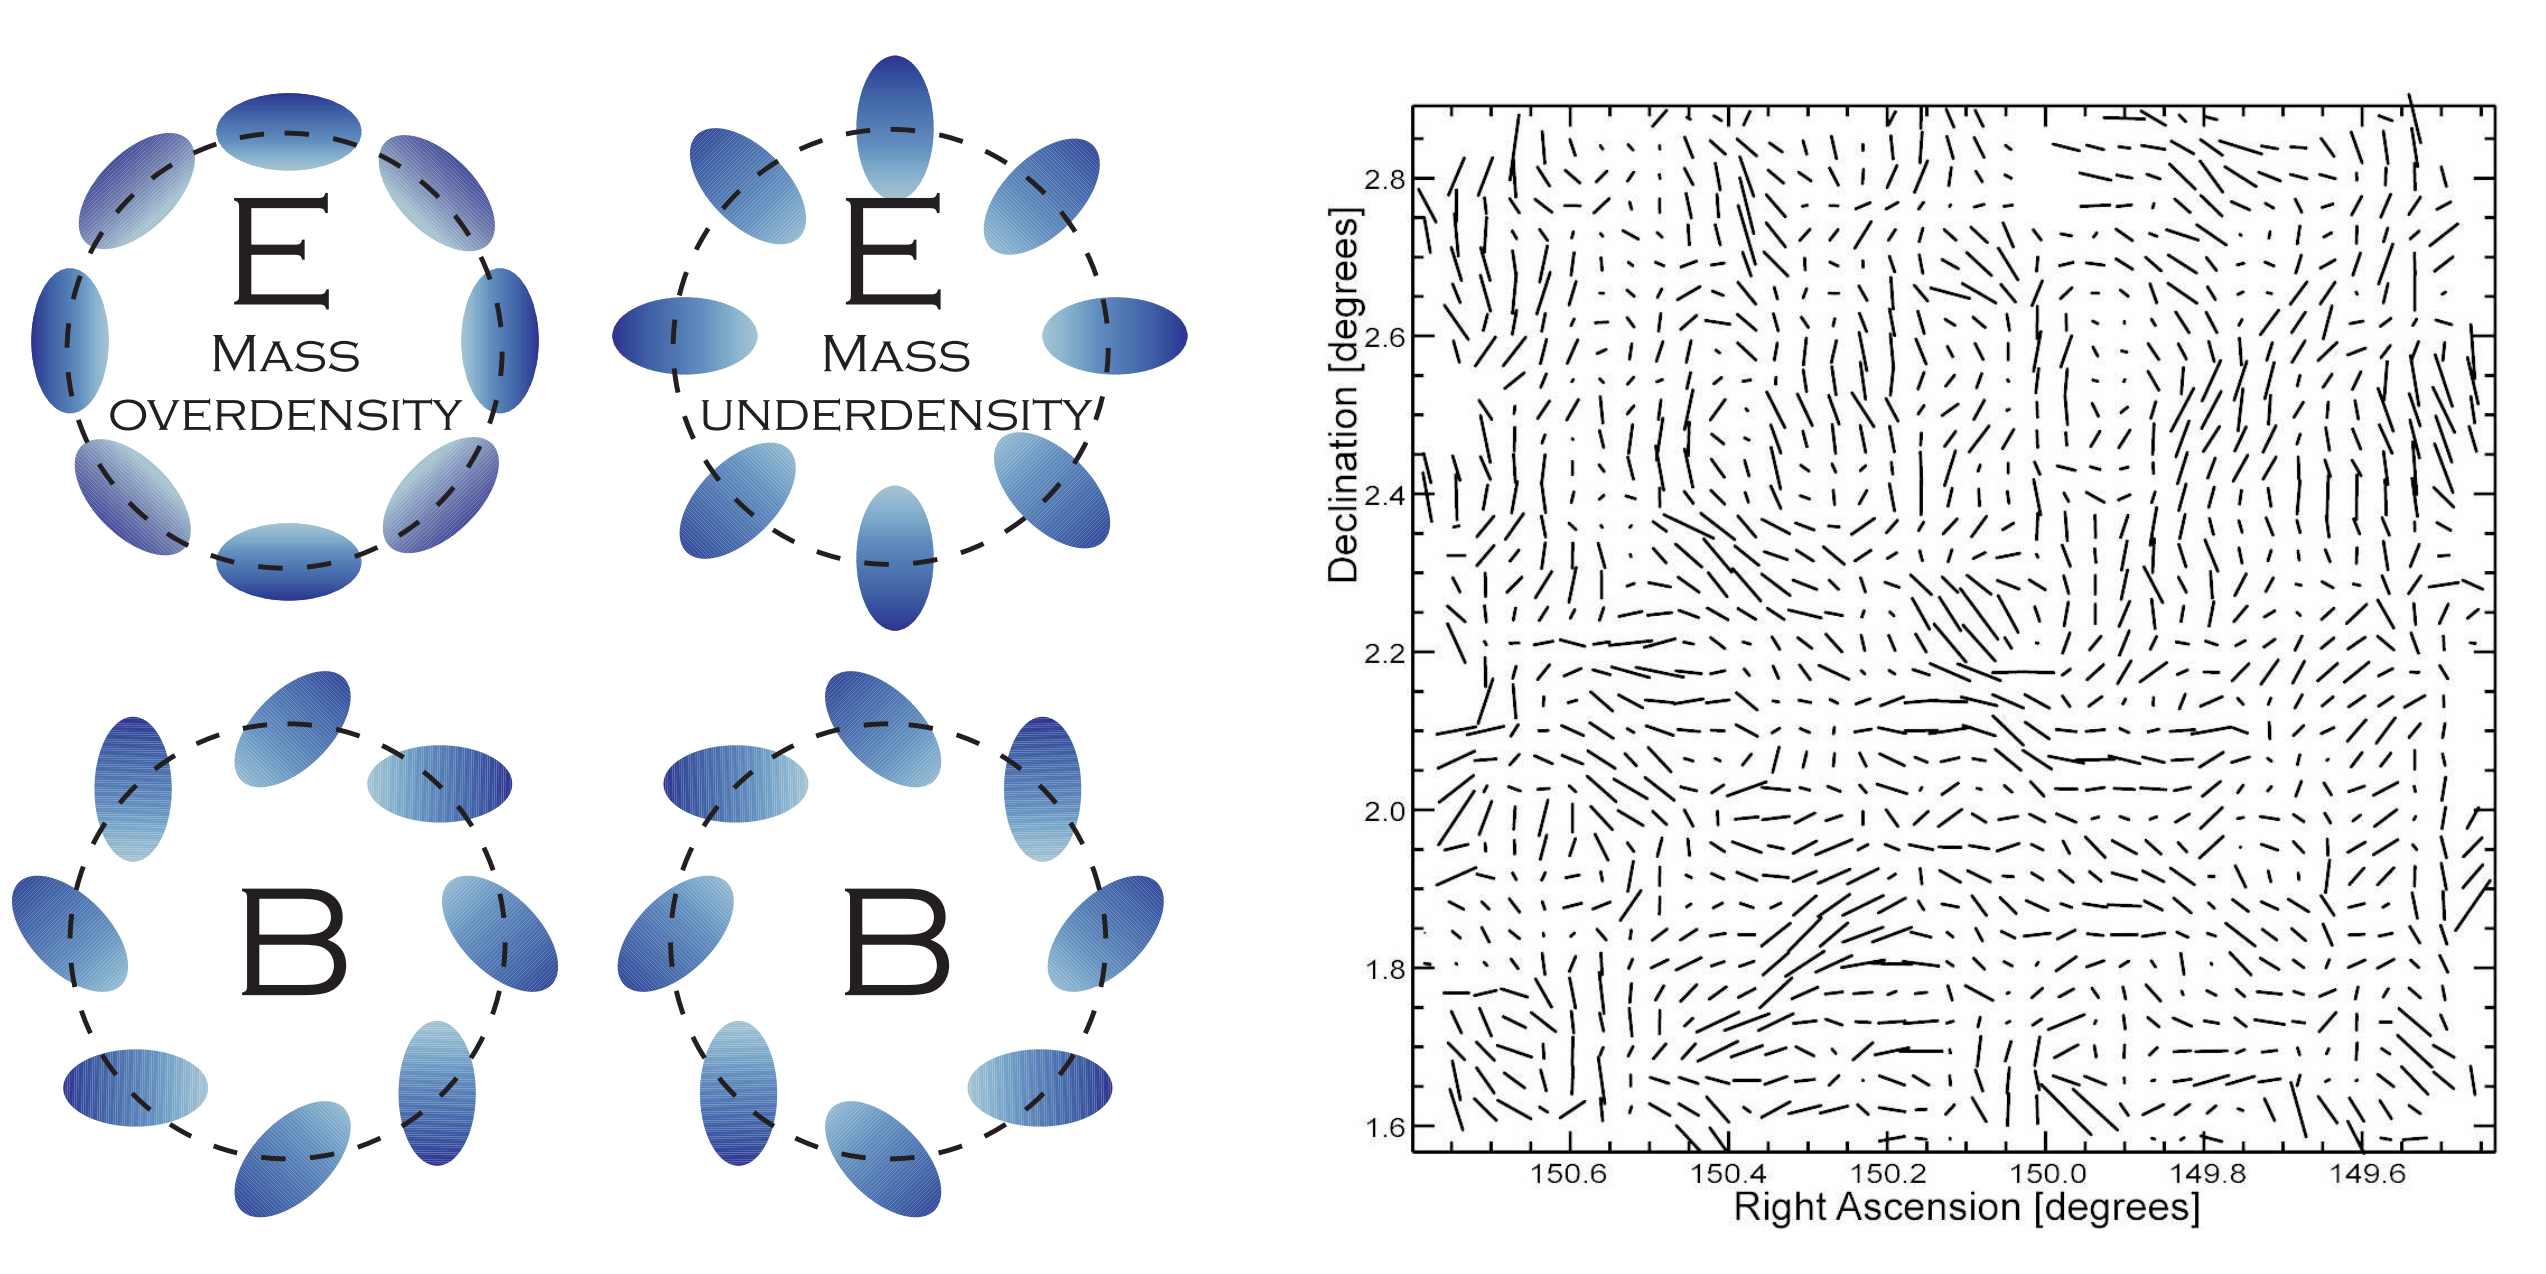
\includegraphics[width=\textwidth]{DarkMatter/Figures/weak_lensing.png}
  \caption{
    Left: Examples of circular ``$E$-mode'' and curl-like ``$B$-mode'' patterns.
    Right: The observed ellipticities of half a million distant galaxies within the 2 square degree Hubble Space Telescope COSMOS survey.
    Reprinted fom Reference~\cite{}. % https://arxiv.org/abs/1001.1739
  }
  \label{fig:weak_lensing}
\end{figure}

The next regime is known as weak lensing, where the deflection is enough to distort the image of the source but not enough to result in multiple images.
The shear of this distortion can be converted into a map of the projected mass distribution.
True weak lensing results in circular ``$E$-mode'' patterns while sources of systematic uncertainty produce both ``$E$-mode'' and curl-like ``$B$-mode'' patterns.
Thus, requiring a zero ``$B$-mode'' contribution assures that the measured mass distribution is accurate.
Figure~\ref{fig:weak_lensing} shows the observed shear of half a million galaxies measured in the Hubble Space Telescope COSMOS survey.

The final regime is the micolensing that occurs when a lens moves relative to a luminous source.
As the lens passes in front of the source, it will temporarily increase the apparent luminosity of the source, enabling a mass measurement of the lens.
Microlensing results show that rocky exoplanets orbit other stars and that these planets cannot form the bulk of dark matter in the Milky Way.

\begin{figure}[htbp]
  \centering
  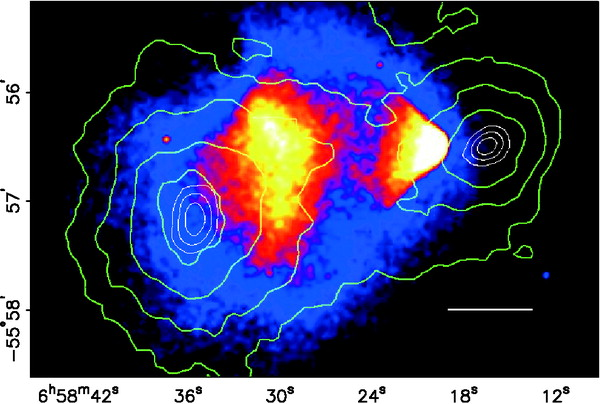
\includegraphics[width=0.75\textwidth]{DarkMatter/Figures/bullet_cluster.jpg}
  \caption{
    The merging cluster 1E0657-558.
    The green contours show the weak lensing reconstruction of the gravitational potential of the cluster.
    The colors indicate the X-ray temperature of the plasma, changing from blue to white as the plasma goes from coolest to hottest.
    The smaller ``bullet'' cluster on the right which traversed through the larger cluster on the left.
    Reprinted from Reference~\cite{}. % https://iopscience.iop.org/article/10.1086/508162
  }
  \label{fig:bullet_cluster}
\end{figure}

\subsection{Cluster Collisions}
\label{sec:dm_bullet}

Additionally, gravitational lensing measurements of galactic cluster collisions provide support for dark matter and help constrain its properties.
Figure~\ref{fig:bullet_cluster} shows the merging cluster 1E0657-558.
By comparing the weak lensing reconstruction of the gravitational potential of the cluster shown in green contours against temperature color gradient of the X-ray emitting interstellar plasma, it was learned that the gravitational potential of the cluster does not track the dominant baryonic mass contribution coming from the plasma.
Instead, the gravitational potential tracks the smaller stellar baryonic mass component.
Dark matter must be the dominant gravitational source in the cluster since the center of total mass is offset from the center of baryonic mass.
Furthermore, the observation of two gravitional mass centers places strong constraints on the self-interaction of dark matter requiring that the observed mass must have a self-interaction collisional cross section $\sigma/m < 1.25\cm^2\text{g}^{-1}$ at a 68\% confidence level.

\section{Relic Density}
\label{sec:dm_relic}

During the early universe, dark matter (DM) was in thermal equilibrium with the rest of the SM particles with a number density $n_\chi$ given by
\begin{equation}
  n_\chi^{\text{eq}} = \frac{g}{(2\pi)^3} \int f(\vec p) \, \text{d}^3 \vec p,
\end{equation}
where $g$ is the number of internal degrees of freedom of the DM particle $\chi$ and $f(\vec p)$ is either the Fermi-Dirac or Bose-Einstein distribution, depending on the quantum statistics of the DM particle.
At very high temperatures relative to the mass $m_\chi$ of the DM particle, dark matter and SM particles rapidly convert back and forth with a DM annihilation rate $\Gamma = \langle \sigma_A v \rangle \cdot n_\chi$, where $\langle \sigma_A v \rangle$ is the thermally averaged product of the total cross section for annihilation $\sigma_A$ and the relative velocity $v$ of the dark matter particles.
After the temperature drops below $m_\chi$, the DM annihilation rate $\Gamma$ drops below the Hubble expansion rate $H$ of the universe and the DM particles stop annihilating and freeze-out of equilibrium with the SM particles, leaving the DM relic density that we observe today.
During the freeze-out process, the time dependence of the number density $n_\chi$ is described by the Boltzmann equation as follows
\begin{equation}
  \frac{\text{d} n_\chi}{\text{d}t} + 3 H n_\chi = - \langle \sigma_A v \rangle \left[ (n_\chi)^2 - (n_\chi^{\text{eq}})^2\right].
\end{equation}
The LHS term accounts for the reduction in density due to the expansion of the universe.
The two RHS terms account for the change in density due to annihilation and product of DM particles to and from SM particles, respectively.

\begin{figure}[htbp]
  \centering
  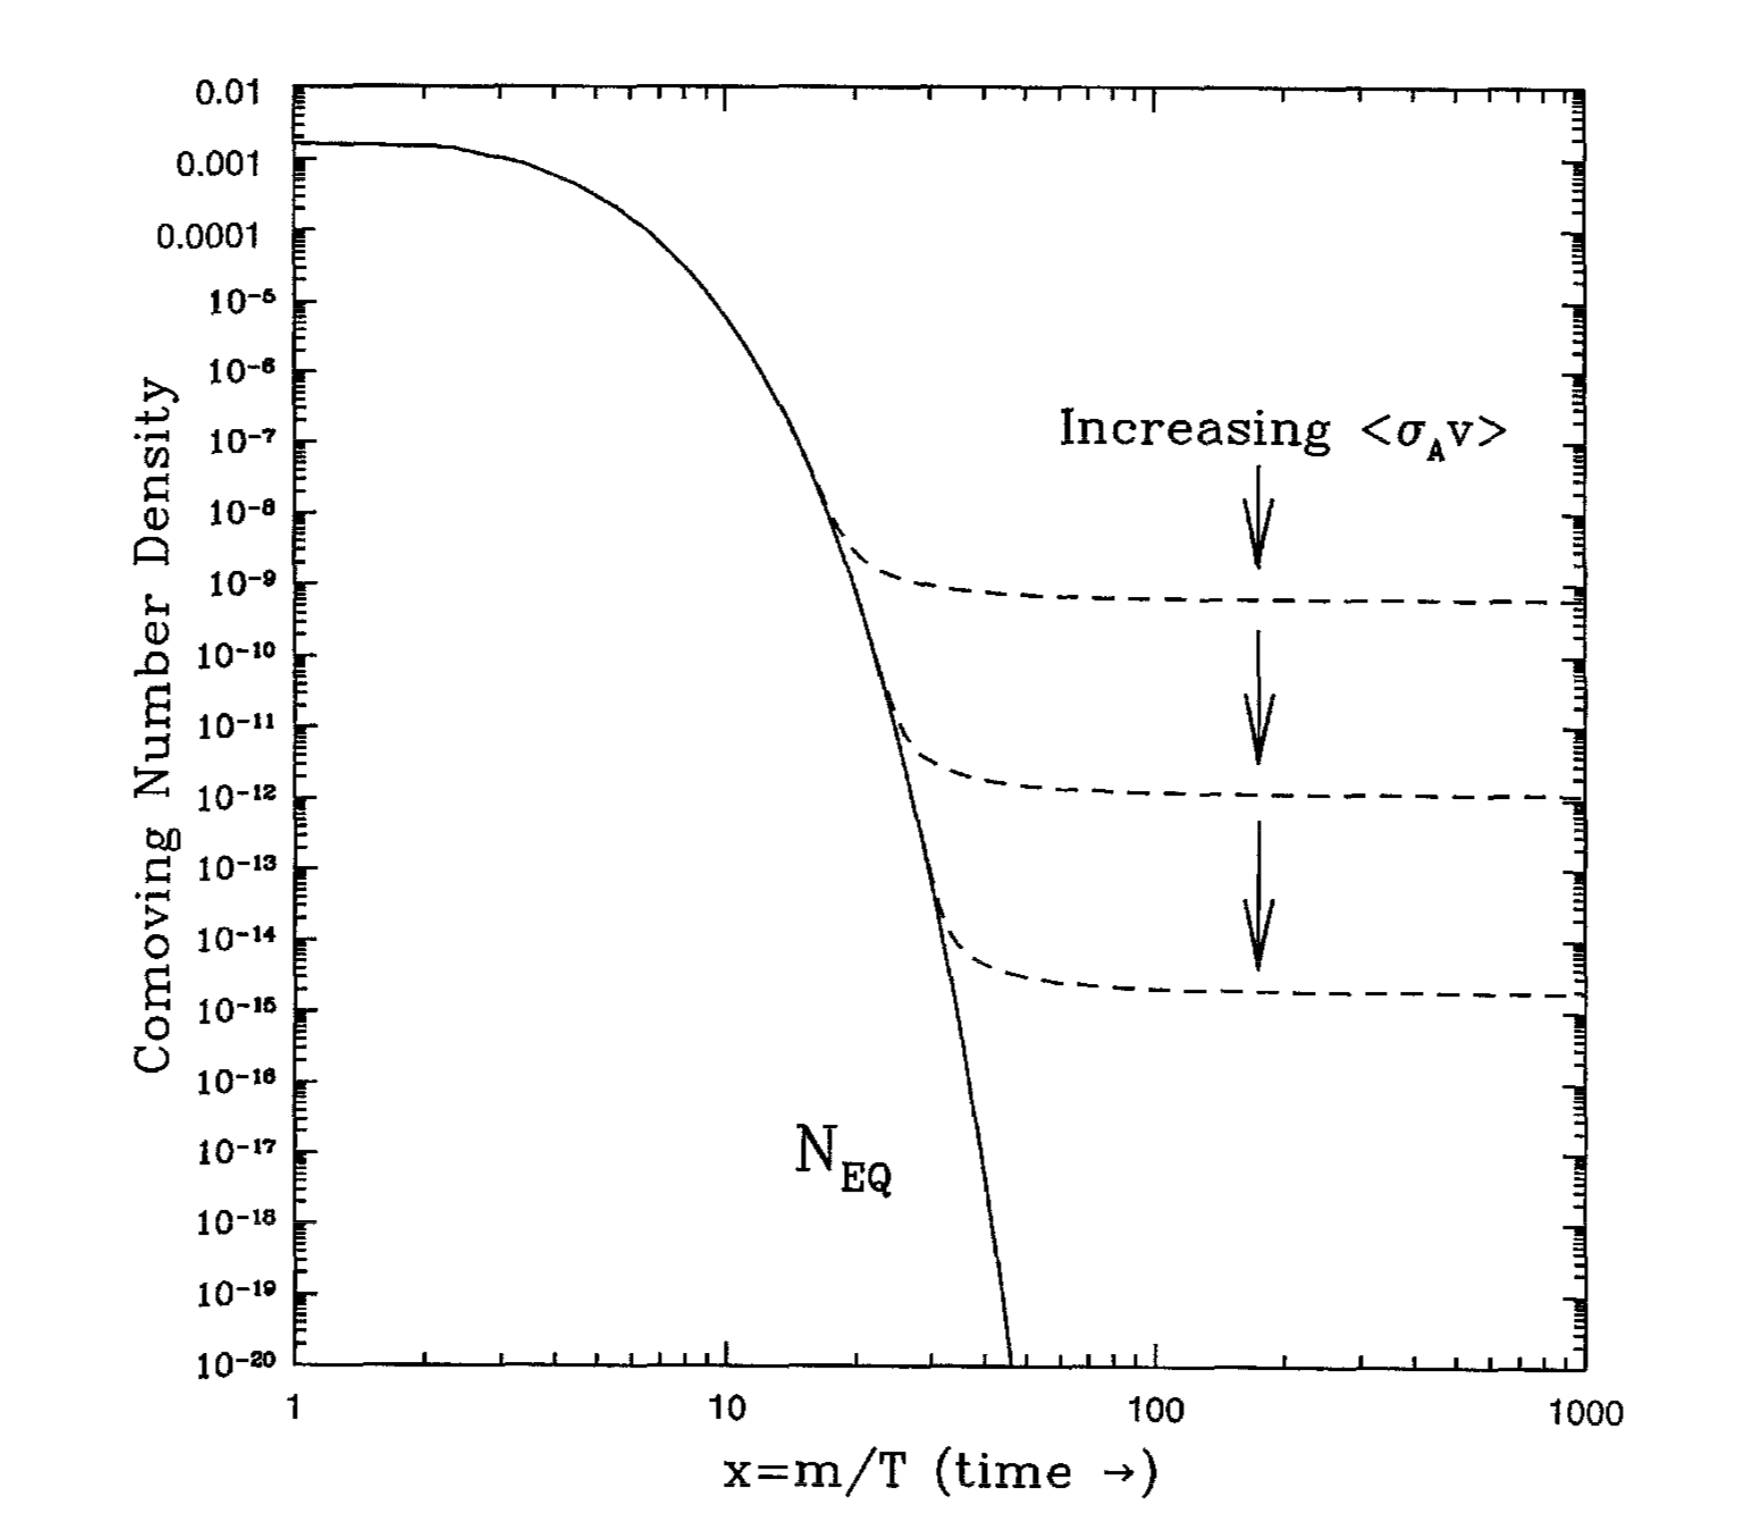
\includegraphics[width=0.625\textwidth]{DarkMatter/Figures/relic_density.png}
  \caption{
    Number density of dark matter in the early universe as a function of time.
    The solid curves are the equilibrium abundance while the dashed curves are the actual abundance after freeze-out.
    Reprinted from Reference~\cite{}. % https://doi.org/10.1016/0370-1573(95)00058-5
  }
  \label{fig:relic_density}
\end{figure}

Figure~\ref{fig:relic_density} shows the calculated DM number density $n_\chi$ as a function of time in the early universe.
As the annihilation cross section increases, the relic density decreases as the dark matter particles stay in equilibrium longer.
We shall make an order-of-magnitude estimate of the relic density by assuming that $\langle \sigma_A v \rangle$ is independent of energy.
Freeze-out occurs at the temperature $T_f$ where the expansion rate $H(T)$ equals the annihilation rate $\Gamma(T)$.
The temperature dependence of $\Gamma$ is simply that of $n_\chi$, e.g. $\Gamma \propto T^3$.
Meanwhile, the early universe is radiation dominated, so we have that $H \propto T^2$. 
Futhermore, astrophysical measurements (see Section~\ref{sec:dm_astro}) can't give direct bounds on the number density, only on the mass density $\rho_\chi = m_\chi n_\chi$. 
Additionally, mass densities are usually expressed as a fraction of the critical density of the universe $\rho_c = 3H^2/(8\pi G)$.
Combining all of this, the relic density of dark matter is given by 
\begin{equation}
  \label{eqn:relic_density}
  \dmrelic = \frac{m_\chi n_\chi}{\rho_c} \simeq \frac{10^{-27} \cm^{3}\text{ s}^{-1}}{\langle \sigma_A v \rangle},
\end{equation}
where $h = H_0/(100 \text{ km s}^{-1}\text{ Mpc}^{-1})$ is the reduced Hubble constant. 
Thus, to first order the DM relic density depends only on two things: the total DM annihilation cross section $\sigma_A$ and the mass $m_\chi$ of the DM candidate, as after freeze-out $T \ll m_\chi$ and the velocity $v$ is stricly proportional to $m_\chi$. 
The latest Planck results measure that $\dmrelic = 0.1200 \pm 0.0012$, providing strong constaints on the possible values of $\sigma_A$ and $m_\chi$.

\section{Dark Matter Candidates}
\label{sec:dm_cand}

Any dark matter candidate must satisfy the following criteria:
\begin{itemize}
\item No or extremely weak interactions with photons, e.g. be \underline{\textbf{\textit{dark}}}
\item Weak baryonic interactions to preserve the DM halos discussed in Section~\ref{sec:dm_curves}
\item Weak self-interactions as discussed in Section~\ref{sec:dm_bullet}
\item The observed relic density discussed in Section~\ref{sec:dm_relic}.
\end{itemize}
These four criteria place stringent requirements on dark matter candidates.
The light neutrinos, the only SM particles satisfying the first three conditions, are excluded as the total neutrino relic density has a bound of $\Omega_\nu \cdot h^2 \leq 0.00067$ at 95\% confidence level from analysis of the CMB anisotropies.
Big Bang Nucleosynthesis and gravitational microlensing have mostly exclude non-luminious baryonic matter from forming the bulk of dark matter.
Thus, most theories of dark matter propose a new fundamental particle as a dark matter candidate.
The following sections discuss the most common dark matter candidates, namely axions, sterile neutrinos, and weakly-interacting massive particles (WIMPs).

\subsection{Axions}
\label{sec:dm_axion}

The hypothetical axion particle introduced in Section~\ref{sec:qcd} is a dark matter candidate if the axion decay constant $f_a$ is large enough as all axion-SM couplings are inversely proportional to it.
Constraints from the observed duration of the neutrino burst from supernova SN 1987A require that $f_a \gtrsim 10^9\GeV$, sufficiently high that the axion lifetime exceeds the age of the universe by many orders of magnitude. % https://arxiv.org/pdf/hep-ph/0611350.pdf
Thus, the axion is a viable DM candidate due to its long lifetime and weak couplings to SM particles.

After accounting for kinematic mixing with the $\pi^0$ and $\eta$ mesons, the axion mass is given by
\begin{equation}
  m_a = \left(\frac{\sqrt{m_u m_d}}{m_u + m_d}\right) \left(\frac{f_\pi}{f_a}\right) m_\pi \simeq \left( \frac{10^7\GeV}{f_a}\right) \eV,
\end{equation}
where $f_\pi$ is the pion decay constant and $m_u$, $m_d$, and $m_\pi$ are the masses of the up quark, the down quark, and the neutral pion, respectively.
From this, we see that the axion mass is inversely proportional to $f_a$, leading to an upper limit of $m_a \lesssim 10 \meV$.
The Planck measurements of the cosmic microwave background also provide a lower (upper) bound on the axion mass $m_a \gtrsim 10 \mueV$ (axion decay constant $f_a \lesssim 10^{12}\GeV$), otherwise the axion abundance is too high.

The axion obtains a two-photon vertex through loops involving virtual quarks and gluons of the form
\begin{equation}
  \mathcal{L}_{a\gamma\gamma} = \frac{1}{4} g_{a\gamma\gamma} \epsilon_{\mu\nu\rho\sigma} F^{\mu\nu} F^{\rho\sigma} a = - g_{a\gamma\gamma} \left(\vec E \cdot \vec B\right) a,
\end{equation}
where $F^{\mu\nu}$ is the electromagnetic field-strength tensor, $\vec E$ and $\vec B$ are the electric and magnetic fields, respectively, and the coupling constant is
\begin{equation}
  g_{a\gamma\gamma} = - \frac{\alpha}{3\pi f_a} \left( \frac{m_u + 4m_d}{m_u + m_d}\right).
\end{equation}
From this, we can see that the axion's coupling to the photon is incredibly small unless in the presence of a strong electromagnetic field.
Thus, astrophysical axions are \underline{\textbf{\textit{dark}}} unless they enter a region with such a field.
Searches for axions such as CAST\cite{} and ADMX\cite{} exploit this to try to observe axion-to-photon conversions.

\subsection{Weakly-Interacting Massive Particles}
\label{sec:dm_wimp}

The annihilation cross-section of new particle $\chi$ with electroweak scale interactions is approximately
\begin{equation}
  \langle \sigma_A v \rangle \approx \left( \frac{\alpha \cdot g_\chi^2}{m_\chi} \right)^2 = \left( \frac{e^2}{4\pi} \cdot \frac{(0.8)^2}{100\GeV} \right)^2 \simeq 10^{-26} \cm^{3}\text{ s}^{-1},
\end{equation}
where $\alpha = e^2 / 4\pi$ is the fine-structure constant, $m_\chi = 100\GeV$ is the mass of the particle, and $g_\chi \approx 0.8$ is the effective coupling for the four-point interaction $\chi \bar\chi \rightarrow f \bar f$.
Plugging this into Equation~\ref{eqn:relic_density}, we obtain $\dmrelic \sim 0.1$, which is very close to the observed value.
This numerical coincidence motivates a new weakly-interacting massive particle (WIMP) as a good DM candidate.

The only criteria to be a WIMP beyond the generic definition of dark matter is that the mass and interaction strength of the new particle must be approximately that of the EWK scale.
Thus, a great many new physics models have WIMPS natively, such as the neutralino in supersymmetry and the lightest Kaluza-Klein particle in theories of universal extra dimensions.
In this thesis, we shall focus on a set of simplified models that describe WIMP interactions in a relatively model-independent manner. For more details, see Section~\ref{sec:dm_simp}.

\section{Non-collider Searches}
\label{sec:dm_search}

Describes.

\section{Simplified Models for LHC}
\label{sec:dm_simp}

It was the hot thing at the time.
